\documentclass[a4paper,11pt]{exam}
%\printanswers % pour imprimer les réponses (corrigé)
\noprintanswers % Pour ne pas imprimer les réponses (énoncé)
\addpoints % Pour compter les points
% \noaddpoints % pour ne pas compter les points
%\qformat{\textbf{\thequestion ) } }
%\qformat{\textbf{\thequestion )}} % Pour définir le style des questions (facultatif)
\usepackage{color} % définit une nouvelle couleur
\shadedsolutions % définit le style des réponses
% \framedsolutions % définit le style des réponses
\definecolor{SolutionColor}{rgb}{0.8,0.9,1} % bleu ciel
\renewcommand{\solutiontitle}{\noindent\textbf{Solution:}\par\noindent} % Définit le titre des solutions
\usepackage{gensymb}



\makeatletter

\def\maketitle{{\centering%
	\par{\huge\textbf{\@title}}%
	\par{\@date}%
	\par}}


\renewcommand{\thesubsection}{\Alph{subsection}.}   

\makeatother

\lhead{NOM Pr\'enom :}
\rhead{\textbf{Les r\'eponses doivent \^etre justifi\'ees et r\'edig\'ees}}
\cfoot{\thepage / \pageref{LastPage}}


%\usepackage{../../pas-math}
%\usepackage{../../moncours}


%\usepackage{pas-cours}
%-------------------------------------------------------------------------------
%          -Packages nécessaires pour écrire en Français et en UTF8-
%-------------------------------------------------------------------------------
\usepackage[utf8]{inputenc}
\usepackage[frenchb]{babel}
%\usepackage{numprint}
\usepackage[T1]{fontenc}
%\usepackage{lmodern}
\usepackage{textcomp}
\usepackage[french, boxed]{algorithm2e}
\usepackage{hyperref}


%-------------------------------------------------------------------------------

%-------------------------------------------------------------------------------
%                          -Outils de mise en forme-
%-------------------------------------------------------------------------------
\usepackage{hyperref}
\hypersetup{pdfstartview=XYZ}
%\usepackage{enumerate}
\usepackage{graphicx}
\usepackage{multicol}
\usepackage{tabularx}
\usepackage{multirow}
\usepackage{color}
\usepackage{eurosym}


\usepackage{anysize} %%pour pouvoir mettre les marges qu'on veut
%\marginsize{2.5cm}{2.5cm}{2.5cm}{2.5cm}

\usepackage{indentfirst} %%pour que les premier paragraphes soient aussi indentés
\usepackage{verbatim}
\usepackage{enumitem}
\usepackage{booktabs}
\usepackage[usenames,dvipsnames,svgnames,table]{xcolor}

\usepackage{variations}

%-------------------------------------------------------------------------------


%-------------------------------------------------------------------------------
%                  -Nécessaires pour écrire des mathématiques-
%-------------------------------------------------------------------------------
\usepackage{amsfonts}
\usepackage{amssymb}
\usepackage{amsmath}
\usepackage{amsthm}
\usepackage{tikz}
\usepackage{xlop}
\usepackage[output-decimal-marker={,}]{siunitx}
%-------------------------------------------------------------------------------

%-------------------------------------------------------------------------------
%                  -Nécessaires pour écrire des formules chimiquess-
%-------------------------------------------------------------------------------

\usepackage[version=4]{mhchem}

%-------------------------------------------------------------------------------
% Pour pouvoir exploiter les fichiers directement dans beamer
\newcommand{\pause}{\ }
%-------------------------------------------------------------------------------
%                    - Mise en forme avancée
%-------------------------------------------------------------------------------

\usepackage{ifthen}
\usepackage{ifmtarg}


\newcommand{\ifTrue}[2]{\ifthenelse{\equal{#1}{true}}{#2}{$\qquad \qquad$}}

%\newcommand{\kword}[1]{\textcolor{red}{\underline{#1}}}
%-------------------------------------------------------------------------------

%-------------------------------------------------------------------------------
%                     -Mise en forme d'exercices-
%-------------------------------------------------------------------------------
%\newtheoremstyle{exostyle}
%{\topsep}% espace avant
%{\topsep}% espace apres
%{}% Police utilisee par le style de thm
%{}% Indentation (vide = aucune, \parindent = indentation paragraphe)
%{\bfseries}% Police du titre de thm
%{.}% Signe de ponctuation apres le titre du thm
%{ }% Espace apres le titre du thm (\newline = linebreak)
%{\thmname{#1}\thmnumber{ #2}\thmnote{. \normalfont{\textit{#3}}}}% composants du titre du thm : \thmname = nom du thm, \thmnumber = numéro du thm, \thmnote = sous-titre du thm

%\theoremstyle{exostyle}
%\newtheorem{exercice}{Exercice}
%
%\newenvironment{questions}{
%\begin{enumerate}[\hspace{12pt}\bfseries\itshape a.]}{\end{enumerate}
%} %mettre un 1 à la place du a si on veut des numéros au lieu de lettres pour les questions 
%-------------------------------------------------------------------------------

%-------------------------------------------------------------------------------
%                    - Mise en forme de tableaux -
%-------------------------------------------------------------------------------

\renewcommand{\arraystretch}{1.7}

\setlength{\tabcolsep}{1.2cm}

%-------------------------------------------------------------------------------



%-------------------------------------------------------------------------------
%                    - Racourcis d'écriture -
%-------------------------------------------------------------------------------
%Droites
\newcommand{\dte}[1]{$(#1)$}
\newcommand{\fig}[1]{figure $#1$}
\newcommand{\sym}{symétrique}
\newcommand{\syms}{symétriques}
\newcommand{\asym}{axe de symétrie}
\newcommand{\asyms}{axes de symétrie}
\newcommand{\seg}[1]{$[#1]$}
\newcommand{\monAngle}[1]{$\widehat{#1}$}
\newcommand{\bissec}{bissectrice}
\newcommand{\mediat}{médiatrice}
\newcommand{\ddte}[1]{$[#1)$}


% Angles orientés (couples de vecteurs)
\newcommand{\aopp}[2]{(\vec{#1}, \vec{#2})} %Les deuc vecteurs sont positifs
\newcommand{\aopn}[2]{(\vec{#1}, -\vec{#2})} %Le second vecteur est négatif
\newcommand{\aonp}[2]{(-\vec{#1}, \vec{#2})} %Le premier vecteur est négatif
\newcommand{\aonn}[2]{(-\vec{#1}, -\vec{#2})} %Les deux vecteurs sont négatifs

%Ensembles mathématiques
\newcommand{\naturels}{\mathbb{N}} %Nombres naturels
\newcommand{\relatifs}{\mathbb{Z}} %Nombres relatifs
\newcommand{\rationnels}{\mathbb{Q}} %Nombres rationnels
\newcommand{\reels}{\mathbb{R}} %Nombres réels
\newcommand{\complexes}{\mathbb{C}} %Nombres complexes


%Intégration des parenthèses aux cosinus
\newcommand{\cosP}[1]{\cos\left(#1\right)}
\newcommand{\sinP}[1]{\sin\left(#1\right)}


%Probas stats
\newcommand{\stat}{statistique}
\newcommand{\stats}{statistiques}


\newcommand{\homo}{homothétie}
\newcommand{\homos}{homothéties}


\newcommand{\mycoord}[3]{(\textcolor{red}{\num{#1}} ; \textcolor{Green}{\num{#2}} ; \textcolor{blue}{\num{#3}})}
%-------------------------------------------------------------------------------

%-------------------------------------------------------------------------------
%                    - Mise en page -
%-------------------------------------------------------------------------------

\newcommand{\twoCol}[1]{\begin{multicols}{2}#1\end{multicols}}


\setenumerate[1]{font=\bfseries,label=\textit{\alph*})}
\setenumerate[2]{font=\bfseries,label=\arabic*)}


%-------------------------------------------------------------------------------
%                    - Elements cours -
%-------------------------------------------------------------------------------

%Correction d'exercice
\newcommand{\exoSec}[2]{\subsection*{Exercice #1 page #2}}
%-------------------------------------------------------------------------------
%                    - raccourcis d'écriture -
%-------------------------------------------------------------------------------

%Mise en évidence de termes clés
\newcommand{\mykw}[1]{\textcolor{red}{\underline{\textbf{#1}}}}

%Exercices
\newcommand{\exo}[2]{exercice #1 page #2}
\newcommand{\Exo}[2]{Exercice #1 page #2}

\renewcommand{\pause}{\ }

%Intervalles
\newcommand{\interOO}[2]{$]$#1 , #2$[$}
\newcommand{\interOF}[2]{$]$#1 , #2$]$}
\newcommand{\interFO}[2]{$[$#1 , #2$[$}
\newcommand{\interFF}[2]{$[$#1 , #2$]$}



%\usepackage{fullpage}
\author{\ }
\date{19 Octobre 2018}
\title{Sciences Physiques : DS n° 2}


\begin{document}
%	\usepackage{fancyhdr}
%	
%	\pagestyle{fancy}
%	\fancyhf{}
	%\rhead{Share\LaTeX}

	\maketitle
	
\begin{small}
	\begin{center}
		\begin{tabular}{|@{\ }l@{}|@{\ }c@{\ }|}
			\hline
			\textbf{Compétence} & \textbf{Maitrise} \\
			\hline
			Caractériser les différents états de la matière (solide, liquide et gaz)\ &  \ \ \ \\
			\hline	
			Espèce chimique et mélange\ &  \ \ \ \\
			\hline
		\end{tabular}
	\end{center}
\end{small}	
	
	
%\vspace*{-0.5cm}	

%\section{\'Equations de réaction}

Ajuster les équations de réactions suivantes :
\begin{questions}
	\question $CH_4 + ....O_2 \rightarrow ....CO_2 + ....H_2O$
	
	\question $C_7H_{16} + ....O_2 \rightarrow ....CO_2 + ....H_2O$	
	
	\question $C_6H_{2}O + ....O_2 \rightarrow ....CO_2 + ....H_2O$
\end{questions}


%\section{À chaque modèle sa formule}
\begin{questions}
	\question \'A partir de ces dessins de modèles, donner la formule des molécules suivantes.

	\begin{center}
		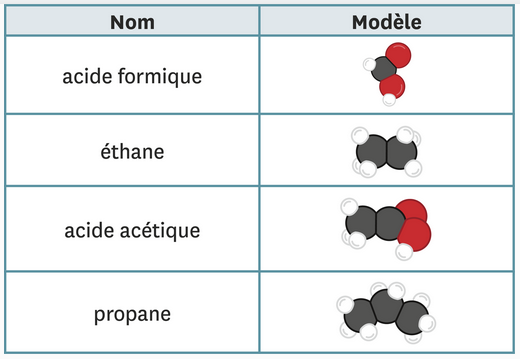
\includegraphics[scale=0.6]{img/exemples}
	\end{center}
	\fillwithdottedlines{2cm}
	
\end{questions}

Seul l'\ref{ex:prod} est à faire sur le sujet. Le soin et la qualité de rédaction sont pris en compte dans la notation.

\section{Source d'énergie renouvelable}\label{ex:renouvelable}

Donner la définition d'une source d'énergie renouvelable ainsi qu'un exemple.

\begin{solution}
	Une source d'énergie renouvelable est une source d'énergie que l'on peut utiliser de manière illimitée à l'échelle humaine. Le vent est une source d'énergie renouvelable.
\end{solution}

\section{Production d'électricité}\label{ex:prod}

L'impact de la production d'électricité sur notre environnement dépend du type de centrale électrique utilisée.
Remplir chaque case avec la bonne réponse.

\begin{center}
	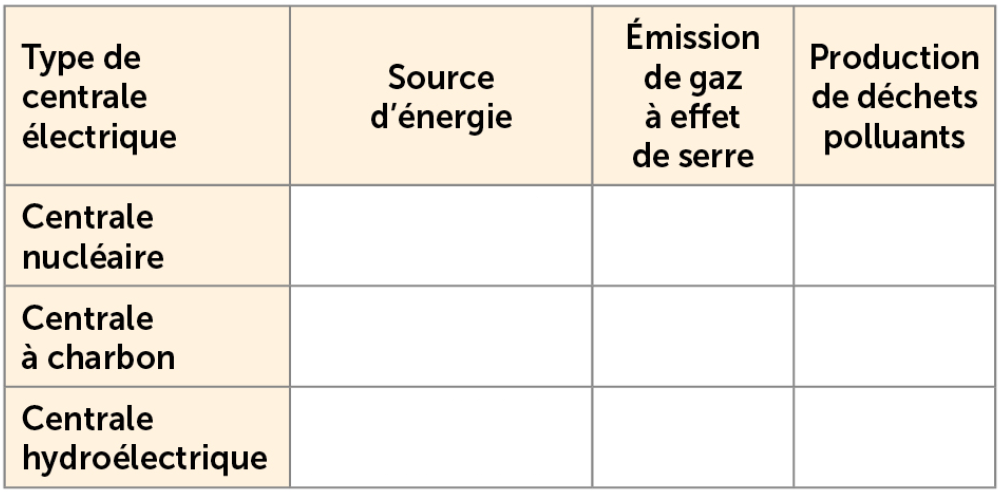
\includegraphics[scale=0.5]{img/tab_centrales}
\end{center}

\section{Surf}\label{ex:surf}

\begin{questions}
	\question Quelle source d'énergie est utilisée par le surfeur pour avancer ?
	
	\question Cette source d'énergie est-elle renouvelable ou non renouvelable ?
\end{questions}

%\section{Parasol}\label{ex:parasol}

\begin{questions}
	\question Pourquoi Oscar aura-t-il moins chaud s'il se met sous le parasol ?
	
	\question Par quelle expression scientifique pourrait-on remplacer le mot <<chaleur>> ?
\end{questions}
%\newpage

\section{Conversions d'énergie}\label{ex:conversion}

\begin{questions}
	\question Quelle conversion d'énergie est réalisée par une éolienne ? par un ventilateur électrique ?
		\begin{solution}
			Une éolienne convertit l'énergie cinétique en énergie électrique. Un ventilateur convertit l'énergie électrique en énergie cinétique.
		\end{solution}
	
	\question Réaliser la chaine énergétique correspondant à l'éolienne.
		\begin{solution}
			\begin{center}
				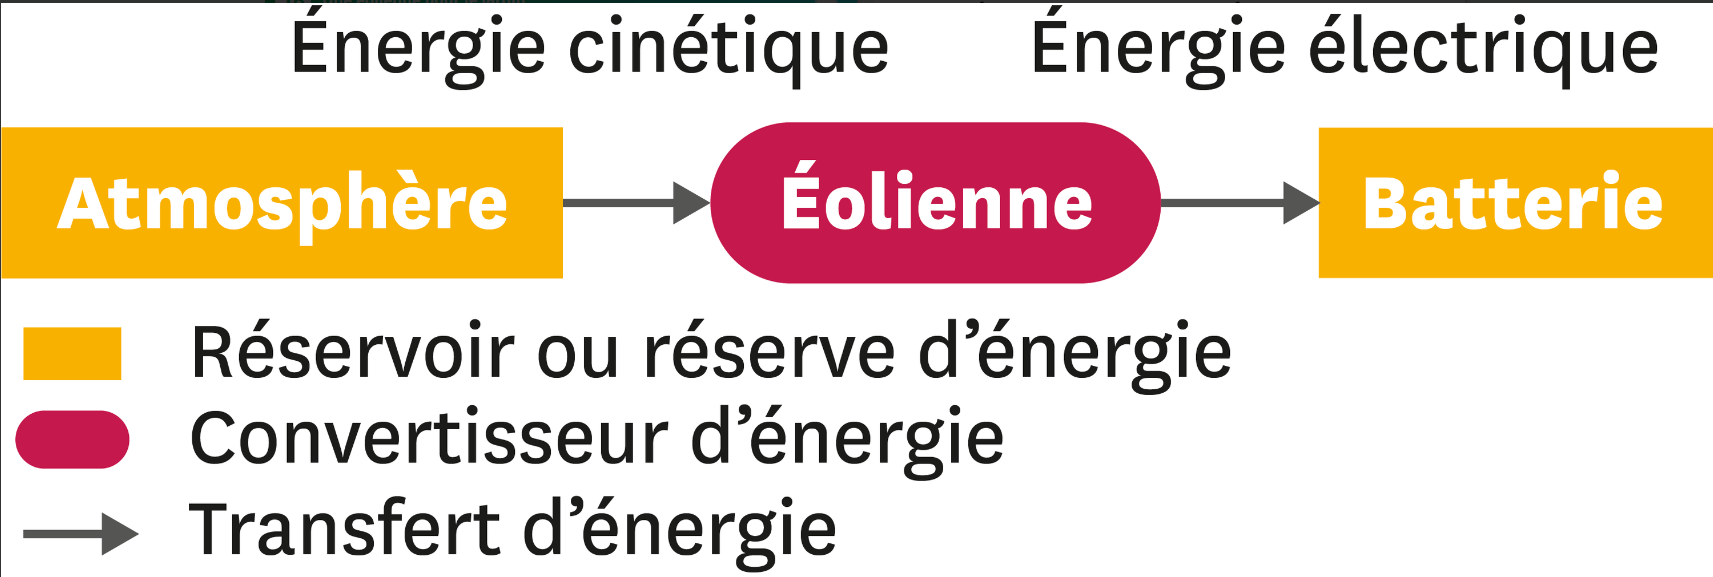
\includegraphics[scale=0.2]{img/chaine}
			\end{center}
		\end{solution}
	
\end{questions}

\section{Une éolienne dans le jardin}\label{ex:eolienne}
	
Julie a installé une éolienne dans son jardin pour son éclairage extérieur. On a symbolisé le fonctionnement de l'éolienne par une chaîne énergétique.

\begin{center}
	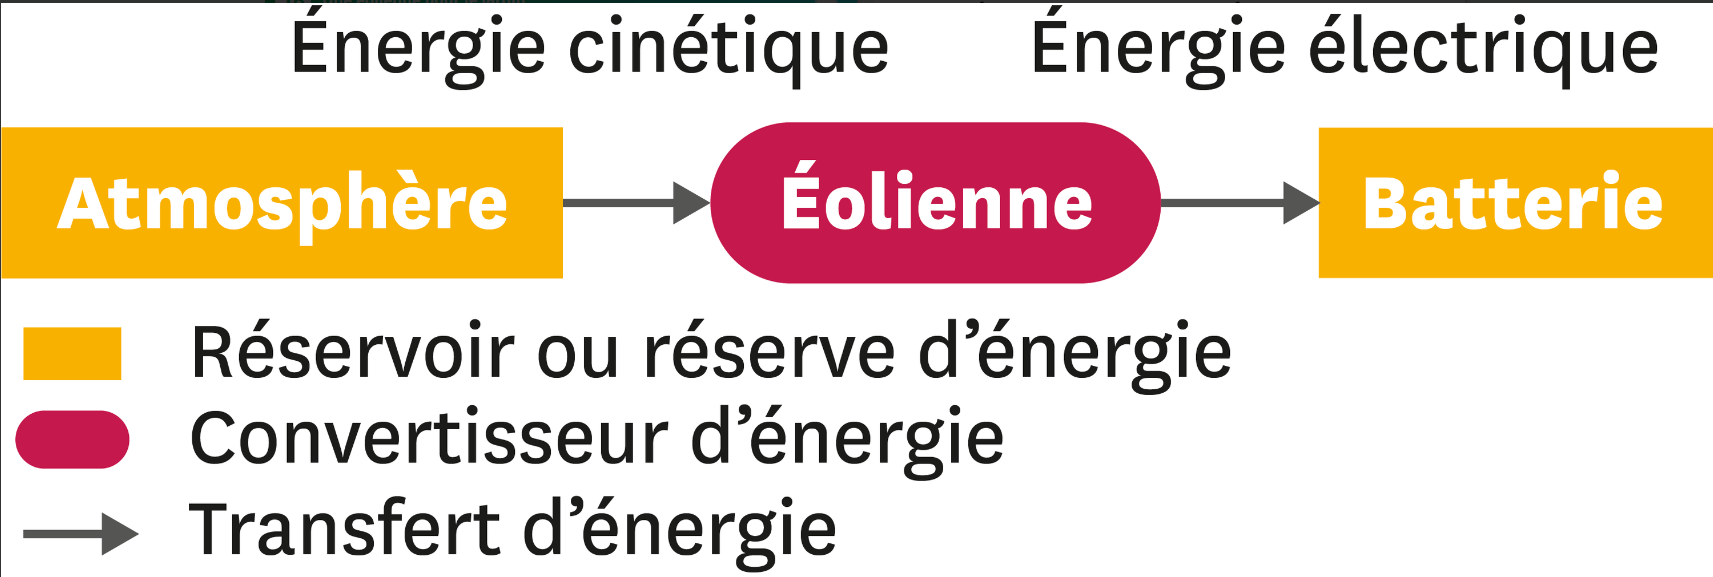
\includegraphics[scale=0.2]{img/chaine}
\end{center}

\begin{questions}
	\question Quel est le réservoir d'énergie qui transmet de l'énergie à l'éolienne ?
	
	\question Quelle forme d'énergie est transmise à l'éolienne ?
	
	
	\question Quel est le réservoir d'énergie qui reçoit de l'énergie de la part de l'éolienne ?
	
	\question Sous quelle forme se fait le transfert d'énergie de l'éolienne vers le réservoir final ?
\end{questions}

\section{Le train à vapeur}\label{ex:train}

Les premiers train fonctionnaient grâce à des moteurs à vapeur. 
L'énergie stockée dans l'air et 
dans le charbon était transférée au moteur à vapeur sous forme d'énergie thermique.
Le moteur convertissait ensuite l'énergie reçue en énergie de mouvement qu'il transférait à l'ensemble du train. On considère que le charbon et l'air font partie d'un seul et même  réservoir d'énergie.

\begin{questions}
	\question Quels étaient les deux réservoirs d'énergie et le convertisseur d'énergie ?
		\begin{solution}
			Les deux réservoirs d'énergie sont d'une part celui formé par l'air et le charbon et d'autre part l'ensemble du train. Le moteur est le convertisseur.
		\end{solution}
	
	\question Le moteur convertissait l'énergie qu'il recevait en une autre forme d'énergie. Laquelle ?
		\begin{solution}
			Le moteur reçoit de l'énergie thermique et la convertit en énergie de mouvement.
		\end{solution}
	
	\question Réaliser la chaine énergétique du fonctionnement de ce train. 
		\begin{solution}
			\begin{center}
				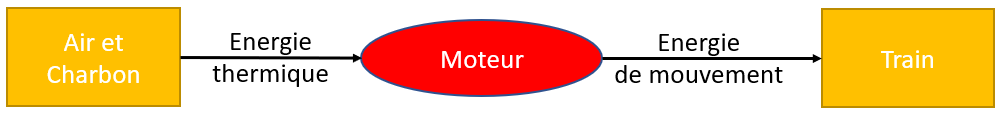
\includegraphics[scale=0.6]{img/chaine_train}
			\end{center}
		\end{solution}
		
\end{questions}

\section{Comparaison de combustibles}\label{ex:comparaison}

\begin{center}
	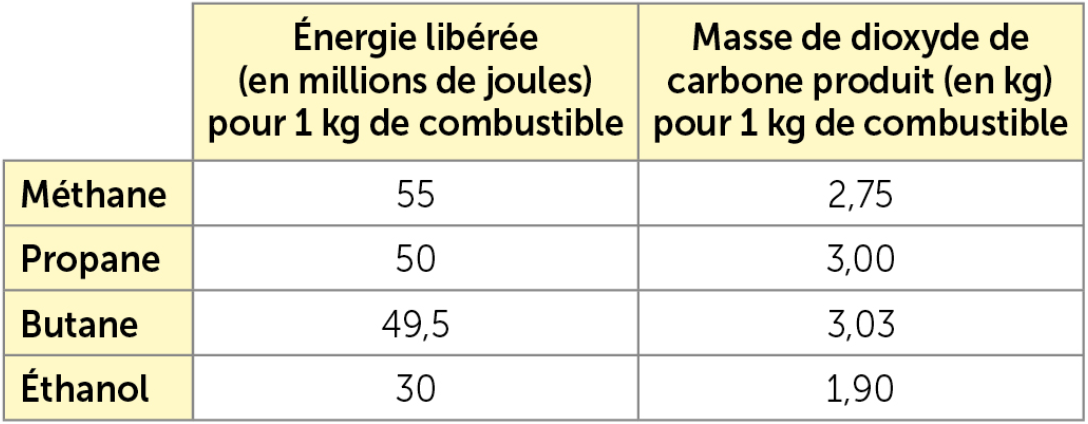
\includegraphics[scale=0.5]{img/tab_combustibles}
\end{center}

\begin{questions}
	\question Quel est le combustible le plus rentable énergiquement ?
	
	\question Sachant que le dioxyde de carbone est un gaz à effet de serre qui contribue au réchauffement climatique, quel combustible est le plus écologique ?
	
	\question Calculer la quantité d'énergie libérée par la combustion de 60 kg de propane et la masse de dioxyde de carbone produit.
\end{questions}

 
%\newpage
%
%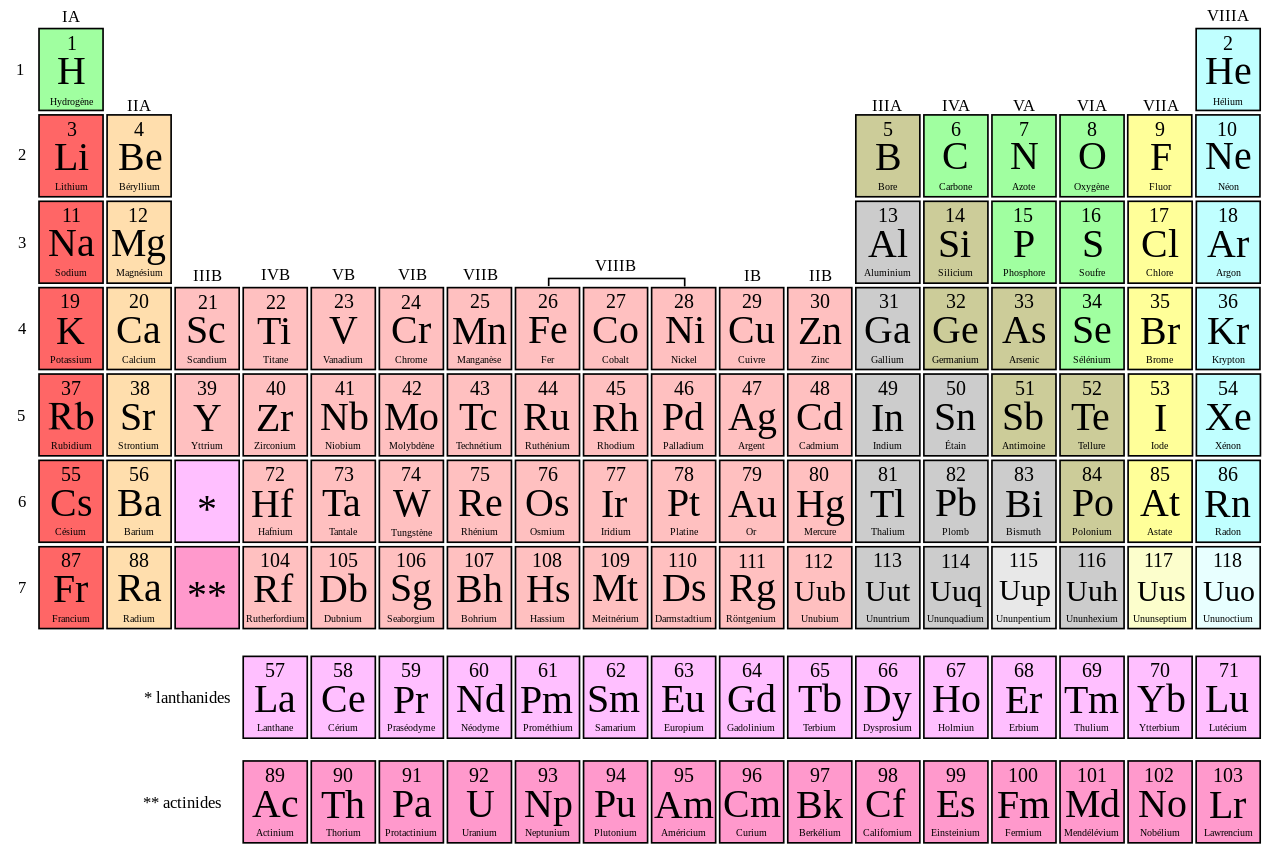
\includegraphics [scale=0.5, angle= 90 ]{img/tableau} 
\ \label{LastPage}

\end{document}